% SC2002 --- Chapter 3: Inheritance & Polymorphism (0->100 ground-up)
\chapter{Inheritance \& Polymorphism: Reuse Without Copy-Paste}
\label{ch:inheritance}

\begin{quote}
\emph{``Inheritance is not for reuse---reuse is a consequence. Inheritance is for polymorphism.''} --- Copy-paste is the enemy; inheritance and polymorphism let us vary behaviour while honouring a common contract.
\end{quote}

\noindent\fbox{\parbox{\dimexpr\linewidth-2\fboxsep-2\fboxrule}{%
\textbf{From zero: built on Ch.~1--2.} We define \emph{inheritance}, \emph{subtyping}, \emph{overriding}, \emph{dynamic dispatch}, and \emph{polymorphism} from scratch. No prior inheritance experience assumed.}}
\vspace{0.4em}

\section*{Learning Outcomes}
After this chapter you will be able to:
\begin{enumerate}[label=(L\arabic*)]
    \item model generalisation/specialisation with inheritance and distinguish \texttt{extends} vs.\ subtyping;
    \item override methods correctly, apply \texttt{super}, and explain dynamic dispatch (late binding);
    \item contrast overloading (compile-time) vs.\ overriding (runtime) and abstract classes vs.\ interfaces;
    \item apply Liskov Substitution Principle informally (subtype must be usable as supertype);
    \item decide when to prefer composition over inheritance.
\end{enumerate}

% ============================================================
\section{Generalisation and Inheritance}
\label{sec:generalisation}
Many domain concepts share structure: \texttt{Book}, \texttt{EBook}, \texttt{AudioBook} all have title/author/id; e-books add download links, audiobooks add duration. Rather than duplicating fields, we factor the common part into a \emph{superclass}.

\begin{figure}[h]
\centering
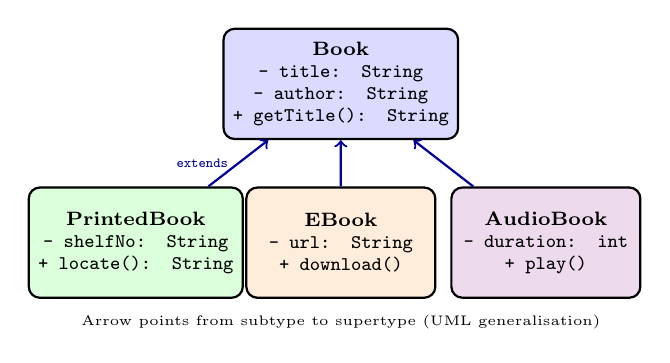
\begin{tikzpicture}[scale=0.84, every node/.style={font=\scriptsize}]
\tikzset{cls/.style={draw,thick,minimum width=2.4cm,minimum height=1.4cm,align=center,rounded corners=4pt}}
\node[cls,fill=blue!14] (sup) at (4.0,1.6) {\textbf{Book}\\\texttt{- title: String}\\\texttt{- author: String}\\\texttt{+ getTitle(): String}};
\node[cls,fill=green!14] (a) at (0.9,-0.8) {\textbf{PrintedBook}\\\texttt{- shelfNo: String}\\\texttt{+ locate(): String}};
\node[cls,fill=orange!14] (b) at (4.0,-0.8) {\textbf{EBook}\\\texttt{- url: String}\\\texttt{+ download()}};
\node[cls,fill=violet!14] (c) at (7.1,-0.8) {\textbf{AudioBook}\\\texttt{- duration: int}\\\texttt{+ play()}};
\draw[->,thick,blue!60!black] (a) -- (sup) node[midway,left,font=\tiny] {\texttt{extends}};
\draw[->,thick,blue!60!black] (b) -- (sup);
\draw[->,thick,blue!60!black] (c) -- (sup);
\node[font=\tiny,fill=white,rounded corners=2pt,inner sep=2pt] at (4.0,-2.0) {Arrow points from subtype to supertype (UML generalisation)};
\end{tikzpicture}
\caption{Inheritance factors common state/behaviour into a superclass; subclasses specialise by adding fields/methods or overriding behaviour.}
\label{fig:inheritance-generalisation}
\end{figure}

\begin{definition}[Inheritance and Subtyping]
\emph{Inheritance} is a language mechanism where a subclass reuses/extends a superclass's members. \emph{Subtyping} is the type relationship: every instance of the subclass is also an instance of the supertype ($S <: T$), so it may be used wherever $T$ is expected.
\end{definition}

Java: \texttt{class EBook extends Book \{ ... \}}. The subclass inherits accessible fields/methods, may add new ones, and may \emph{override} inherited methods with a more specific implementation. Constructors are not inherited---each class constructs its own part via \texttt{super(...)}.

\begin{lstlisting}[language=Java, caption={Inheritance with constructor chaining and overriding.}]
public class Book {
    protected String title; protected String author;
    public Book(String title, String author) { this.title=title; this.author=author; }
    public String description() { return title + " by " + author; }
}
public class EBook extends Book {
    private String url;
    public EBook(String t, String a, String url) { super(t,a); this.url=url; }
    @Override public String description() { return super.description() + " [eBook: " + url + "]"; }
    public void download() { /* ... */ }
}
\end{lstlisting}

% --- TikZ 2: Dynamic dispatch / vtable ---
\begin{figure}[h]
\centering
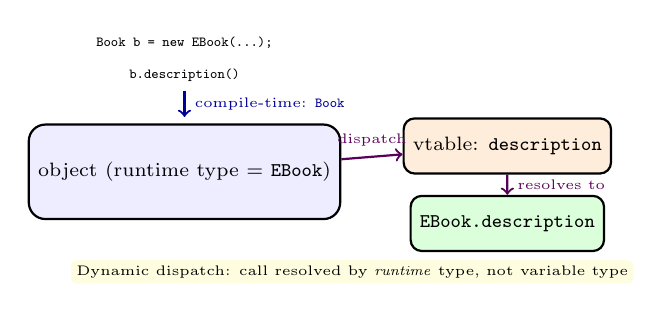
\begin{tikzpicture}[scale=0.82, every node/.style={font=\scriptsize}]
\node[font=\tiny,align=center] at (0,2.1) {\texttt{Book b = new EBook(...);}};
\node[font=\tiny,align=center] at (0,1.6) {\texttt{b.description()}};
\draw[->,thick,blue!60!black] (0,1.35) -- (0,0.95) node[midway,right,font=\tiny] {compile-time: \texttt{Book}};
\node[draw,thick,fill=blue!7,rounded corners=6pt,minimum width=3.8cm,minimum height=1.2cm] (obj) at (0,0.1) {object (runtime type = \texttt{EBook})};
\node[draw,thick,fill=orange!14,rounded corners=4pt,minimum width=2.2cm,minimum height=0.7cm] (vt) at (5.0,0.5) {vtable: \texttt{description}};
\node[draw,thick,fill=green!14,rounded corners=4pt,minimum width=2.2cm,minimum height=0.7cm] (impl) at (5.0,-0.7) {\texttt{EBook.description}};
\draw[->,thick,violet!70!black] (obj) -- (vt) node[midway,above,font=\tiny] {dispatch};
\draw[->,thick,violet!70!black] (vt) -- (impl) node[midway,right,font=\tiny] {resolves to};
\node[font=\tiny,fill=yellow!12,rounded corners=2pt,inner sep=2pt] at (2.6,-1.45) {Dynamic dispatch: call resolved by \emph{runtime} type, not variable type};
\end{tikzpicture}
\caption{Dynamic dispatch (late binding): the method invoked depends on the object's actual class at runtime.}
\label{fig:dynamic-dispatch}
\end{figure}

\section{Polymorphism and Dynamic Dispatch}
\label{sec:polymorphism}
\emph{Polymorphism} (``many forms'') means one interface, many implementations. In Java, a variable of type \texttt{Book} may hold any subtype instance; calling \texttt{description()} executes the subtype's override. This is \emph{dynamic dispatch} (late binding).

Why it matters: code that works with \texttt{Book} need not know which subtype it has. Adding \texttt{AudioBook} requires no changes to loan logic that calls \texttt{book.description()}---open for extension, closed for modification (preview of Ch.~5).

\paragraph{Overloading vs.\ overriding.} Overloading: same name, different parameters, resolved at compile time. Overriding: same signature, subclass replaces behaviour, resolved at runtime. Missing \texttt{@Override} hides bugs silently---always annotate.

\subsection{Abstract Classes and Interfaces}
An \emph{abstract} class cannot be instantiated; it may declare abstract methods (no body) that subclasses must implement. An \emph{interface} is a pure contract (no state, only method signatures + default/static helpers since Java 8). Prefer interfaces for ``can-do'' roles (e.g., \texttt{Borrowable}, \texttt{Payable}); use abstract classes when subclasses share state and common implementation.

\begin{lstlisting}[language=Java, caption={Interface as contract; multiple behaviours via polymorphism.}]
public interface Borrowable { boolean isAvailable(); void markBorrowed(); }
public abstract class LibraryItem implements Borrowable {
    protected String id; protected boolean available = true;
    public boolean isAvailable() { return available; }
    public abstract String description(); // each subtype describes differently
}
public class Book extends LibraryItem {
    private String title;
    public Book(String id, String t) { this.id=id; this.title=t; }
    public void markBorrowed() { available=false; }
    public String description() { return "Book: " + title; }
}
\end{lstlisting}

% --- TikZ 3: Composition vs Inheritance ---
\begin{figure}[h]
\centering
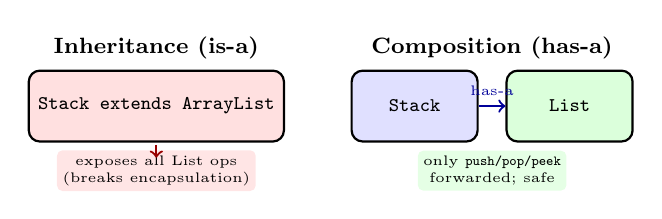
\begin{tikzpicture}[scale=0.82, every node/.style={font=\scriptsize}]
\begin{scope}
\node[font=\footnotesize\bfseries] at (1.4,1.35) {Inheritance (is-a)};
\node[draw,thick,fill=red!12,rounded corners=4pt,minimum width=2.6cm,minimum height=0.9cm] (sa) at (1.4,0.45) {\texttt{Stack extends ArrayList}};
\node[font=\tiny,align=center,fill=red!10,rounded corners=2pt,inner sep=2pt] at (1.4,-0.55) {exposes all List ops\\(breaks encapsulation)};
\draw[->,thick,red!60!black] (1.4,-0.15) -- (1.4,-0.35);
\end{scope}
\begin{scope}[xshift=5.2cm]
\node[font=\footnotesize\bfseries] at (1.4,1.35) {Composition (has-a)};
\node[draw,thick,fill=blue!12,rounded corners=4pt,minimum width=1.6cm,minimum height=0.9cm] (st) at (0.2,0.45) {\texttt{Stack}};
\node[draw,thick,fill=green!14,rounded corners=4pt,minimum width=1.6cm,minimum height=0.9cm] (li) at (2.6,0.45) {\texttt{List}};
\draw[->,thick,blue!60!black] (st) -- (li) node[midway,above,font=\tiny] {has-a};
\node[font=\tiny,align=center,fill=green!10,rounded corners=2pt,inner sep=2pt] at (1.4,-0.55) {only \texttt{push/pop/peek}\\forwarded; safe};
\end{scope}
\end{tikzpicture}
\caption{Prefer composition over inheritance when you want reuse without exposing the reused type's full interface.}
\label{fig:composition-over-inheritance}
\end{figure}

\section{Composition Over Inheritance and LSP}
\label{sec:composition-lsp}
Inheritance couples subclass to superclass implementation. If the superclass changes, subclasses break (fragile base class problem). Guideline: use inheritance only for true \emph{is-a} with behavioural substitutability.

\begin{definition}[Liskov Substitution Principle --- informal]
If $S$ is a subtype of $T$, objects of $T$ should be replaceable by objects of $S$ without breaking correctness. Overridden methods must honour the supertype's contract (preconditions no stronger, postconditions no weaker).
\end{definition}

Classic violation: \texttt{Square extends Rectangle} with \texttt{setWidth} that also sets height---code expecting independent width/height breaks. Fix: do not force that hierarchy; model \texttt{Shape} with separate subtypes or use composition.

\begin{remark}[Checklist: inheritance or composition?]
Is it truly is-a and will callers use the subtype as the supertype? Does the subclass need to override behaviour (polymorphism)? If either answer is no, prefer composition (has-a) with delegation.
\end{remark}

\section{Abstract Classes, Interfaces, and Sealed Hierarchies}
\label{sec:abstract-interfaces}
\paragraph{When to use which.} Start with an interface for a role; introduce an abstract class when multiple implementors share state or common code. Java lets a class implement many interfaces but extend one class---so prefer interfaces for flexibility, abstract classes for code sharing.

\paragraph{Template Method (preview of Ch.~6).} An abstract class can define a skeleton algorithm calling abstract steps that subclasses fill in---the classic way to share control flow while varying details.

\begin{lstlisting}[language=Java, caption={Template Method via abstract class.}] 
public abstract class LoanPolicy {
    public final boolean canBorrow(Member m, Book b){ // skeleton
        return isAvailable(b) && withinLimit(m) && noOverdue(m);
    }
    protected abstract boolean isAvailable(Book b);
    protected abstract boolean withinLimit(Member m);
    protected abstract boolean noOverdue(Member m);
}
\end{lstlisting}

\paragraph{Sealed classes (Java 17+).} \texttt{sealed class Shape permits Circle, Rectangle} lets the compiler know all subtypes, enabling exhaustive \texttt{switch} with no default---a safer closed hierarchy when the set of variants is fixed.

\subsection{Overriding Rules and the Fragile Base Class}
Overriding must match signature and not narrow visibility; \texttt{@Override} makes the compiler enforce it. The fragile-base-class problem: a superclass change (e.g., adding a method that happens to match a subclass method) can silently alter behaviour. Mitigations: favour composition (Fig.~\ref{fig:composition-over-inheritance}), make classes \texttt{final} by default and document extension points, prefer interfaces.

\subsection{Interfaces with Defaults and Functional Roles}
Since Java 8, interfaces may carry \texttt{default} methods (shared behaviour) and \texttt{static} helpers. Use defaults sparingly to avoid the diamond problem; prefer abstract classes when defaults need state.

\begin{lstlisting}[language=Java, caption={Interface defaults---shared behaviour without a base class.}]
interface Borrowable {
    boolean isAvailable();
    void markBorrowed();
    default void borrowOrThrow(){
        if (!isAvailable()) throw new IllegalStateException("not available");
        markBorrowed();
    }
}
\end{lstlisting}
Functional interfaces (\texttt{Predicate<T>, Function<T,R>}) plus lambdas often replace single-method Strategy hierarchies with less ceremony---the \emph{idea} (pluggable behaviour) stays, the boilerplate shrinks. Choose explicit Strategy classes when the behaviour is complex or has its own state/tests.

\subsection{Quick Decision Table}
\begin{center}
\small
\begin{tabular}{lll}
\toprule
Need & Prefer & Why \\
\midrule
Share state + common code & abstract class & fields + constructor \\
Pure capability, many implementors & interface & multiple implementation \\
Closed small variant set & sealed class/interface & exhaustive switch \\
One-method pluggable behaviour & functional interface / lambda & less boilerplate \\
\bottomrule
\end{tabular}
\end{center}

\section{Chapter Notes}
Liskov's principle is Liskov (1987) / Liskov \& Wing (1994). Bloch (Effective Java) Item 18: ``Favour composition over inheritance.'' Java's single-class inheritance + multiple-interface implementation balances reuse and complexity; other languages differ (C++ multiple inheritance, Python MRO).

\section{Exercises}
\label{sec:ch03-exercises}
\begin{enumerate}[label=E3.\arabic*, leftmargin=*, itemsep=0.8em]
    \item \textbf{Override vs.\ overload.} Given \texttt{void foo(Book)} and \texttt{void foo(EBook)} overloads vs.\ \texttt{description()} override, predict which is chosen at compile vs.\ runtime and write a test that demonstrates the difference.
    \item \textbf{Dispatch trace.} With \texttt{Book b = new EBook(...); b.description();} explain step-by-step what the compiler checks and what the runtime does. What if \texttt{description} were \texttt{static}?
    \item \textbf{Abstract vs.\ interface.} Model \texttt{Payable} ( Shenanigan: trip fare, library fine, e-commerce order). Should it be an abstract class or interface? Justify with state-sharing and multiple-inheritance needs.
    \item \textbf{LSP violation.} Show why \texttt{Square extends Rectangle} violates LSP with a code snippet that passes for \texttt{Rectangle} but fails for \texttt{Square}. Propose a corrected hierarchy.
    \item \textbf{Composition refactor.} Refactor \texttt{Stack extends ArrayList} to composition. List which methods you expose, how you delegate, and why this is safer under future \texttt{ArrayList} changes.
\end{enumerate}
% End of Chapter 3
